\chapter{Von den Randbedingungen zum Spektrum offener Strings}

\lectureoverview{Unser Ziel ist es, einen offenen String zu quantisieren und zu entscheiden, ob seine Zustände als Teilchen bezeichnet werden können. Der Weg dorthin ist elementar, aber anspruchsvoll. Zunächst behandeln wir die Differential- und Integralrechnung sowie die Fourier-Analyse von Funktionen auf \(0\leq\sigma\leq\pi\). Dann ersetzen wir die Punktförmigkeit durch ein Spektralkriterium für Teilchenverhalten, betrachten erneut die Beschreibung im Grenzfall unendlichen Impulses, in der die transversale Dynamik nichtrelativistisch wird, und bauen den String aus einer Kette leichter Massen und steifer Federn auf. Der kontinuierliche String ist ein Wellensystem mit freien Enden. Seine Neumann-Moden entkoppeln zu harmonischen Oszillatoren mit den Frequenzen \(1,2,3,\ldots\); die Quantisierung ergibt daher ein diskretes Spektrum mit Energielücke. Stringwechselwirkungen zwingen uns schließlich, über offene Strings hinauszugehen: Ein offener String kann seine beiden Endpunkte verbinden und zu einem geschlossenen String werden.}

\section{Differentialrechnung auf dem Intervall des offenen Strings}

In den folgenden Rechnungen werden diskrete Summen immer wieder durch Integrale und Differenzen zwischen benachbarten Punkten durch Ableitungen ersetzt. Es ist sinnvoll, diese Grundlagen vorab festzuhalten, damit sie die physikalischen Überlegungen nicht unterbrechen.

Sei \(x(\sigma)\) eine Funktion auf

\begin{equation}
  0\leq \sigma\leq \pi .
\end{equation}

Die Notation nimmt die Stringtheorie vorweg: \(\sigma\) bezeichnet die Position entlang des Strings, während \(x\) später eine seiner transversalen Koordinaten sein wird. Wir unterteilen das Intervall in \(N\) Teilstücke,

\begin{equation}
  \Delta\sigma=\frac{\pi}{N},
  \qquad
  \sigma_i=i\,\Delta\sigma,
  \qquad
  x_i=x(\sigma_i).
  \label{eq:l02-lattice}
\end{equation}

Für eine glatte Grenzfunktion gilt:

\begin{equation}
  \Delta x_i\equiv x_i-x_{i-1}
  =
  \frac{\partial x}{\partial\sigma}\,\Delta\sigma
  +O\!\left((\Delta\sigma)^2\right),
  \label{eq:l02-difference}
\end{equation}

und die Riemann-Summe wird zu

\begin{equation}
  \sum_i x_i\,\Delta\sigma
  \longrightarrow
  \int_0^\pi x(\sigma)\,d\sigma .
  \label{eq:l02-riemann}
\end{equation}

\begin{figure}[H]
  \centering
  
\includegraphics[width=0.78\textwidth]{lecture_02_figure_01.png}
  \caption{Die Regeln für Differenzen und Riemann-Summen, die wir für den späteren Übergang zum Kontinuum festhalten.}
  \lectureframe{00:04:20}
  \label{fig:l02-calculus-board}
\end{figure}

Dies sind bekannte Definitionen aus der Analysis. Entscheidend ist hier ihre Skalierung: \(\Delta x_i\) liefert einen Faktor \(\Delta\sigma\), während eine Summe bei ihrem Übergang in ein Integral einen inversen Faktor liefert.

\subsection{Dirichlet- und Neumann-Randbedingungen}

Die Fourier-Analyse auf einem endlichen Intervall beginnt mit der Wahl der Randbedingungen. Zwei Fälle werden immer wieder auftreten.

\begin{align}
  \text{Dirichlet:}\qquad
  &x(0)=x(\pi)=0,
  \label{eq:l02-dirichlet}\\
  \text{Neumann:}\qquad
  &\left.\partial_\sigma x\right|_{\sigma=0}
   =
   \left.\partial_\sigma x\right|_{\sigma=\pi}
   =0.
  \label{eq:l02-neumann}
\end{align}

Eine an beiden Enden gehaltene Geigensaite veranschaulicht den Dirichlet-Fall: Ihre Auslenkung verschwindet an den Rändern. Eine Neumann-Funktion muss dort nicht verschwinden; ihre Steigung ist an jedem Rand null. Die beiden charakteristischen Formen sind gemeinsam auf der Tafel zu sehen.

\begin{figure}[H]
  \centering
  \begin{minipage}[t]{0.48\textwidth}
    \centering
    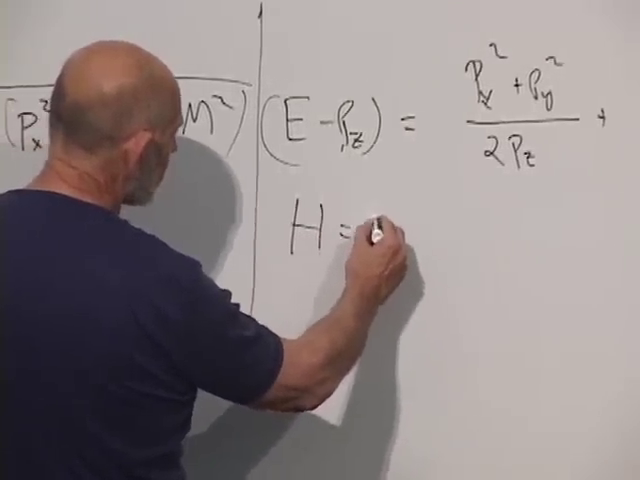
\includegraphics[width=\textwidth]{lecture_02_figure_02.png}
    \par\smallskip\footnotesize (a) Fixierte und am Rand flache Profile.
  \end{minipage}\hfill
  \begin{minipage}[t]{0.48\textwidth}
    \centering
    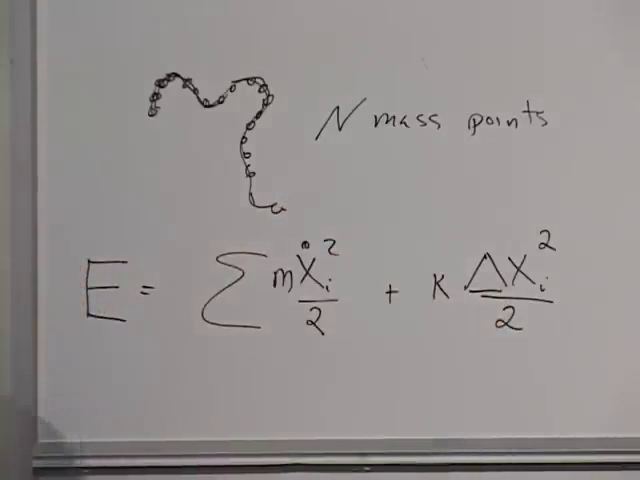
\includegraphics[width=\textwidth]{lecture_02_figure_03.png}
    \par\smallskip\footnotesize (b) Leichte Ringe, die auf vertikalen Stangen gleiten.
  \end{minipage}
  \caption{Randbedingungen als Formen und als mechanische Modelle. Die Konstruktion mit gleitenden Ringen legt die transversale Bewegung eines freien Endes eindeutig fest.}
  \lectureframe{00:08:50 and 00:12:15}
  \label{fig:l02-boundaries-board}
\end{figure}

\begin{figure}[H]
  \centering
  \begin{adjustbox}{max width=\linewidth}
  \begin{tikzpicture}[>=Latex,thick,scale=0.92]
    \begin{scope}
      \draw[->] (0,0) -- (4.4,0) node[right] {\(\sigma\)};
      \draw[->] (0,-1.25) -- (0,1.35) node[above] {\(x\)};
      \draw[blue!70!black]
        (0,0) .. controls (0.8,1.1) and (1.4,1.0) .. (2.0,0)
        .. controls (2.7,-1.0) and (3.4,-0.8) .. (4.1,0);
      \fill (0,0) circle (0.06);
      \fill (4.1,0) circle (0.06);
      \node at (2.05,-1.65) {Dirichlet: \(x=0\)};
    \end{scope}
    \begin{scope}[xshift=5.8cm]
      \draw[->] (0,0) -- (4.4,0) node[right] {\(\sigma\)};
      \draw[->] (0,-1.25) -- (0,1.35) node[above] {\(x\)};
      \draw[orange!85!black]
        (0,0.65) .. controls (0.8,0.65) and (1.1,-0.9) .. (2.0,-0.9)
        .. controls (2.9,-0.9) and (3.2,0.55) .. (4.1,0.55);
      \draw[orange!85!black] (0,0.65) -- (0.45,0.65);
      \draw[orange!85!black] (3.65,0.55) -- (4.1,0.55);
      \node at (2.05,-1.65) {Neumann: \(\partial_\sigma x=0\)};
    \end{scope}
  \end{tikzpicture}
  \end{adjustbox}
  \caption{Beim Dirichlet-Fall ist der Funktionswert festgelegt, beim Neumann-Fall die Steigung.}
  \label{fig:l02-boundaries-redraw}
\end{figure}

\begin{classroomqa}
\audiencequestion{Liefert ein offenes oder geschlossenes Orgelrohr ein anschauliches Beispiel für eine dieser Randbedingungen?\lecturetimestamp{00:09:19}}
\lecturerresponse{Das kann es, aber zunächst muss man angeben, welche akustische Größe entwickelt wird. Druckstörung und longitudinale Auslenkung erfüllen an einem offenen Ende komplementäre idealisierte Randbedingungen. Statt diese Nebenfrage an der Tafel zu klären, verwenden wir das Modell mit den gleitenden Ringen: Nahezu masselose Ringe können sich auf den Stangen vertikal bewegen, sodass die Stringenden frei sind und der Neumann-Fall unmittelbar vorliegt.}
\end{classroomqa}

\begin{classroomqa}
\audiencequestion{Kann der Graph senkrecht ansteigen und einen scharfen Sprung aufweisen?\lecturetimestamp{00:09:53}}
\lecturerresponse{Die Fourier-Analyse lässt isolierte Sprünge in einer stückweise stetigen Funktion zu. Für einen physikalischen String gelten strengere Anforderungen. Ein Sprung trennt benachbarte Punkte voneinander und lässt die räumliche Ableitung \(\partial_\sigma x\) in der weiter unten hergeleiteten Kontinuumsenergie singulär werden. Wir beschränken uns daher auf stetige und differenzierbare Profile.}
\end{classroomqa}

\begin{classroomqa}
\audiencequestion{Warum muss für das offene Ende eines Rohrs oder irgendein freies Ende überhaupt eine Randbedingung gelten?\lecturetimestamp{00:11:14}}
\lecturerresponse{Das akustische Beispiel hängt von der gewählten Feldgröße ab; die Frage blieb in der Diskussion offen. Beim mechanischen Beispiel ist das anders. Ein sehr leichter Ring kann frei gleiten, ist aber weiterhin am letzten Stringsegment befestigt. Wir leiten seine Bedingung aus dem Newtonschen Gesetz her, statt sie vorauszusetzen: Bei endlicher Beschleunigung des Endpunkts muss die Steigung verschwinden.}
\end{classroomqa}

\subsection{Die Fourier-Basen}

Sobald die Randbedingungsklasse feststeht, ist auch die zugehörige Fourier-Basis festgelegt. Auf \(0\leq\sigma\leq\pi\) gilt:

\begin{align}
  x_D(\sigma)
  &=
  \sum_{n=1}^{\infty}x_n\sin(n\sigma),
  \label{eq:l02-dirichlet-series}\\
  x_N(\sigma)
  &=
  \sum_{n=0}^{\infty}x_n\cos(n\sigma).
  \label{eq:l02-neumann-series}
\end{align}

Jeder Sinus in \eqref{eq:l02-dirichlet-series} verschwindet an beiden Endpunkten. Jede Kosinusfunktion in \eqref{eq:l02-neumann-series} hat an den Endpunkten eine Ableitung von null. Die unteren Summationsgrenzen unterscheiden sich aus gutem Grund: \(\sin(0\sigma)=0\) trägt nichts bei, während \(\cos(0\sigma)=1\) die konstante, also nullte, Mode ist. Sie gibt den Mittelwert einer Neumann-Funktion an.

\begin{figure}[H]
  \centering
  \begin{minipage}[t]{0.48\textwidth}
    \centering
    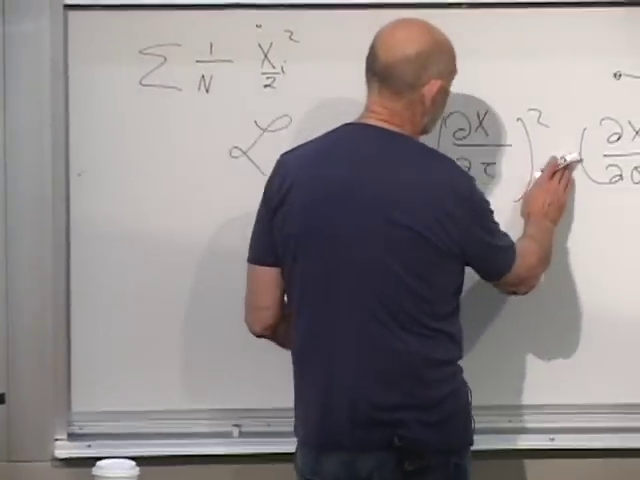
\includegraphics[width=\textwidth]{lecture_02_figure_04.png}
    \par\smallskip\footnotesize (a) Sinus- und Kosinusentwicklungen.
  \end{minipage}\hfill
  \begin{minipage}[t]{0.48\textwidth}
    \centering
    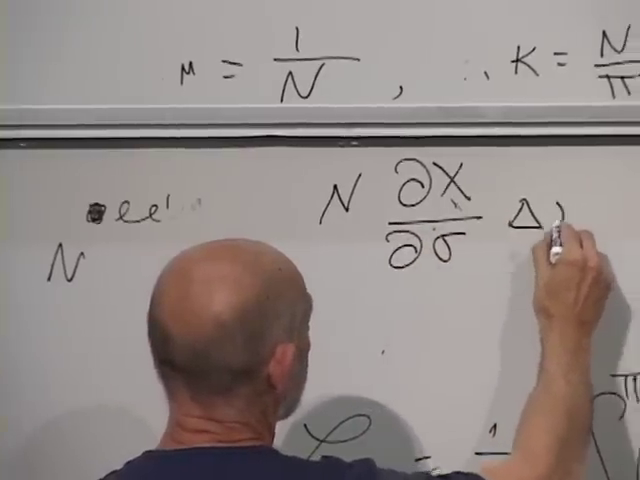
\includegraphics[width=\textwidth]{lecture_02_figure_05.png}
    \par\smallskip\footnotesize (b) Orthogonalität und die besondere konstante Mode.
  \end{minipage}
  \caption{Die Fourier-Eigenschaften, die wir später zur Diagonalisierung des Strings verwenden.}
  \lectureframe{00:16:15 and 00:20:30}
  \label{fig:l02-fourier-board}
\end{figure}

Die Ableitung vertauscht die beiden Klassen:

\begin{equation}
  \begin{aligned}
    \partial_\sigma\sin(n\sigma)&=n\cos(n\sigma),\\
    \partial_\sigma\cos(n\sigma)&=-n\sin(n\sigma).
  \end{aligned}
  \label{eq:l02-basis-derivatives}
\end{equation}

Die Ableitung einer Dirichlet-Reihe hat also Neumann-Verhalten, und die Ableitung einer Neumann-Reihe hat Dirichlet-Verhalten. Durch Orthogonalität verschwinden dann die Kreuzterme zwischen verschiedenen Moden:

\begin{align}
  \int_0^\pi\cos(n\sigma)\cos(m\sigma)\,d\sigma
  &=
  \frac{\pi}{2}\delta_{nm},
  && n,m\geq1,
  \label{eq:l02-cos-orthogonality}\\
  \int_0^\pi\sin(n\sigma)\sin(m\sigma)\,d\sigma
  &=
  \frac{\pi}{2}\delta_{nm},
  && n,m\geq1,
  \label{eq:l02-sin-orthogonality}\\
  \int_0^\pi 1\,d\sigma&=\pi .
  \label{eq:l02-zero-norm}
\end{align}

Die letzte Zeile ist die besondere Kosinusnorm für \(n=m=0\). Eine konstante Funktion wird anders normiert als eine nichtverschwindende Harmonische; dieser Faktor zwei wird die Schwerpunktsmode des Strings von seinen inneren Moden unterscheiden.

\subsection{Eine Oszillatorformel zum Merken}

Nach einer Skalierung der Koordinate, durch die die mechanische Masse auf eins gesetzt wird, gilt für einen harmonischen Oszillator mit Hookeschem Gesetz:

\begin{align}
  E_{\mathrm{osc}}
  &=
  \frac12\dot q^{\,2}
  +\frac12\omega^2q^2,
  \label{eq:l02-oscillator-energy}\\
  L_{\mathrm{osc}}
  &=
  \frac12\dot q^{\,2}
  -\frac12\omega^2q^2.
  \label{eq:l02-oscillator-lagrangian}
\end{align}

\begin{figure}[H]
  \centering
  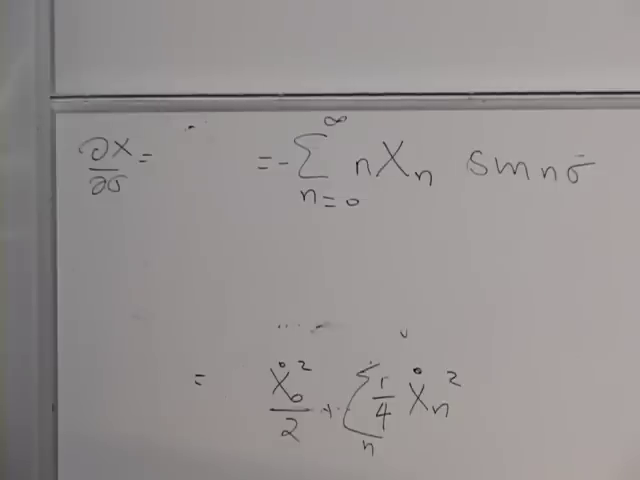
\includegraphics[width=0.68\textwidth]{lecture_02_figure_06.png}
  \caption{Die Energie des Oszillators, so geschrieben, dass der Koeffizient von \(q^2\) unmittelbar \(\omega^2\) erkennen lässt.}
  \lectureframe{00:24:00}
  \label{fig:l02-oscillator-board}
\end{figure}

Klassisch gilt \(\omega=\sqrt{\kappa/m}\); durch die Koordinatenskalierung wurde \(m=1\) gesetzt. In der Quantenmechanik gilt:

\begin{equation}
  E_Q=\hbar\omega\left(Q+\frac12\right),
  \qquad Q=0,1,2,\ldots .
  \label{eq:l02-oscillator-spectrum}
\end{equation}

Für die Abstände zwischen den Energieniveaus können wir den gemeinsamen Grundzustandsterm abziehen und sagen, dass jedes Quant \(\hbar\omega\) kostet. Bei der Stringrechnung verfahren wir zunächst genau so und verschieben die gesamte Nullpunktsenergie auf später.

\begin{classroomqa}
\audiencequestion{Wie liest man die Oszillatorfrequenz aus der Energieformel ab?\lecturetimestamp{00:23:21}}
\lecturerresponse{Vor der Skalierung lautet sie \(\omega=\sqrt{\kappa/m}\). Bei Einheitsmasse ist der Potenzialterm \(\frac12\omega^2q^2\), sein quadratischer Koeffizient ist also das Quadrat der Frequenz.}
\end{classroomqa}

\section{Wann ist ein zusammengesetztes System ein Teilchen?}

Ein String ist ausgedehnt und wird als System vieler gekoppelter Teile modelliert. In welchem Sinn kann einer seiner Quantenzustände dennoch ein Teilchen sein? Punktförmigkeit kann nicht das entscheidende Kriterium sein. Protonen und Neutronen sind zusammengesetzt. Elektronen und Photonen werden von Quantenfeldern begleitet, obwohl bei ihnen keine innere Substruktur aufgelöst wurde. Das Bild eines klassischen geometrischen Punktes, um den herum nichts ist, passt nicht zu einer Quantenanregung.

Auch Masse und Schwerpunktlage reichen als Kriterien nicht aus. Beides hat ein abgeschlossener Gasbehälter. Eine Tasse Kaffee hat beides ebenfalls. Normalerweise würden wir keines von beiden als Teilchen bezeichnen. Auch Unteilbarkeit taugt nicht als Kriterium, denn ein Proton ist teilbar. Und der Spin unterscheidet mikroskopische Teilchen nicht von makroskopischen Körpern.

Ein brauchbares Kriterium ist die Isolation im Spektrum. Tragen wir die Ruheenergie auf einer vertikalen Achse auf und fragen, wie viel Energie erforderlich ist, um einen anderen inneren Zustand zu erreichen. Beim Elektron gibt es keine experimentell zugängliche Folge von Elektronenanregungen unmittelbar oberhalb seines Grundzustands. Beim Proton gibt es zwar Resonanzen, doch die ersten erfordern einige hundert MeV, also einen beträchtlichen Bruchteil der Protonenmasse. Diese Zustände sind weit genug voneinander getrennt, um einzeln identifiziert werden zu können.

Bei einer Tasse Kaffee ist es genau umgekehrt. Man kann einem langwelligen Schallmodus eine beliebig kleine Energiemenge zuführen, ein Molekül anstoßen oder ein Phonon erzeugen. In einem winzigen Energieintervall liegen enorm viele Zustände dicht beieinander. Auf Laborskalen bilden sie ein Kontinuum. Darin liegt der praktische Unterschied zwischen einem Teilchen und \emph{einem Brei}.

\begin{figure}[H]
  \centering
  \includegraphics[width=0.58\textwidth]{lecture_02_figure_07.png}
  \caption{Die vertikale Energieachse an der Tafel vergleicht ein isoliertes Teilchenniveau mit den dicht liegenden Anregungen gewöhnlicher Materie.}
  \lectureframe{00:31:10}
  \label{fig:l02-spectrum-board}
\end{figure}

\begin{figure}[H]
  \centering
  \begin{adjustbox}{max width=\linewidth}
  \begin{tikzpicture}[>=Latex,thick]
    \begin{scope}
      \draw[->] (0,0) -- (0,4.8) node[above] {energy};
      \draw[blue!70!black,line width=1.2pt] (-1.0,0.65) -- (1.0,0.65);
      \draw[blue!70!black,line width=1.2pt] (-1.0,3.65) -- (1.0,3.65);
      \node[right] at (1.05,0.65) {ground state};
      \node[right] at (1.05,3.65) {first internal excitation};
      \draw[<->] (0.65,0.75) -- (0.65,3.55)
        node[midway,right] {large gap};
      \node at (0,-0.55) {particle-like};
    \end{scope}
    \begin{scope}[xshift=7.0cm]
      \draw[->] (0,0) -- (0,4.8) node[above] {energy};
      \foreach \y in {0.55,0.69,0.82,0.94,1.05,1.15,1.24,1.32,1.39,1.45,
        1.51,1.57,1.63,1.70,1.78,1.87,1.97,2.09,2.22,2.36,2.51,2.67,2.84,
        3.02,3.21,3.41,3.62,3.84,4.07}
        \draw[orange!85!black] (-0.95,\y) -- (0.95,\y);
      \node[right] at (1.05,2.25) {dense phonon and internal states};
      \node at (0,-0.55) {macroscopic matter};
    \end{scope}
  \end{tikzpicture}
  \end{adjustbox}
  \caption{Für das Teilchenkriterium in dieser Vorlesung ist die Isolation im Spektrum maßgeblich, nicht die wörtliche Punktförmigkeit.}
  \label{fig:l02-particle-redraw}
\end{figure}

Mit diesem Kriterium wird aus der philosophischen Frage eine Rechnung. Wir quantisieren den String, bestimmen seine inneren Energieniveaus und untersuchen ihre Abstände. Liegt der erste angeregte Stringzustand nahe der Planck-Skala, während der beobachtete Grundzustand leicht ist, übersteigt die Lücke die derzeit erreichbaren Beschleunigerenergien um mehr als zwanzig Größenordnungen. Im gesamten zugänglichen Energiebereich verhält sich der String dann wie ein Elementarteilchen.

\begin{classroomqa}
\audiencequestion{Ist Teilchenverhalten lediglich eine Frage der beobachteten Skala? Verschwinden die getrennten Niveaus, wenn wir weit genug hineinzoomen?\lecturetimestamp{00:33:33}}
\lecturerresponse{Durch Hineinzoomen kann sich zeigen, dass ein Objekt aus vielen Bestandteilen besteht; sein Spektrum wird dadurch aber nicht ausgelöscht. Entscheidend ist der Vergleich zwischen der Energieauflösung des Experiments und der Lücke zur ersten inneren Anregung. Ein zusammengesetztes Objekt kann sich weiterhin wie ein Teilchen verhalten, wenn diese Lücke enorm groß ist.}
\end{classroomqa}

\begin{classroomqa}
\audiencequestion{Warum ist eine gewöhnliche Geigensaite kein Teilchen?\lecturetimestamp{00:34:37}}
\lecturerresponse{Die Energie eines einzelnen Schwingungsquants ist im Vergleich zur Ruheenergie der makroskopischen Saite unmessbar klein. Daher passen sehr viele Quantenzustände in ein winziges relatives Energieintervall. Die Saite gehört in diesem Spektralvergleich zur dicht besetzten, nicht zur isolierten Seite.}
\end{classroomqa}

\begin{classroomqa}
\audiencequestion{Sind Photonen und Elektronen Punktteilchen, wenn Quantenfelder sie mit virtuellen Fluktuationen umgeben?\lecturetimestamp{00:35:40}}
\lecturerresponse{Das klassische Wort \emph{Punkt} übernimmt hier zu viele Aufgaben. Das physikalische Elektron und Photon sind bekleidete Feldanregungen; dennoch haben Experimente bei keinem von beiden eine innere Zusammensetzung oder einen endlichen Formfaktor nachgewiesen. Für das gegenwärtige Argument ist entscheidend, dass keines von beiden eine dichte Folge nahezu entarteter innerer Zustände besitzt.\editorialnote{In der Vorlesung wird das anomale magnetische Moment des Elektrons mit einer messbaren quantenmechanischen Unschärfe in Verbindung gebracht. Nach heutiger Terminologie ist das anomale Moment ein Effekt der Strahlungskorrekturen und kein Beleg für einen aufgelösten endlichen Elektronenradius. „Punktförmig“ bedeutet üblicherweise, dass bis zur untersuchten Skala keine innere Substruktur und kein Formfaktor nachgewiesen wurde.}}
\end{classroomqa}

\begin{classroomqa}
\audiencequestion{Hängt die Größe eines Photons von seiner Frequenz ab?\lecturetimestamp{00:36:49}}
\lecturerresponse{Seine Wellenlänge hängt davon ab. Das ist etwas anderes als eine intrinsische Größe seiner Bestandteile. Eine Änderung der Frequenz verändert das Wellenpaket und die Wellenlänge, nicht aber einen aufgelösten inneren Radius des Photons.}
\end{classroomqa}

\section{Exakte transversale Mechanik bei großem Impuls}

Kehren wir nun zum relativistischen Problem zurück. Ein schnell rotierender Stab lässt sich nicht allein dadurch nichtrelativistisch behandeln, dass man seinen Schwerpunkt in Ruhe setzt. Seine Enden bewegen sich relativ zueinander weiterhin relativistisch. Die nichtrelativistische Näherung versagt wegen der inneren Relativbewegung.

Es gibt jedoch einen anderen Grenzfall. Wir wählen eine \(z\)-Achse und versetzen das gesamte System durch einen Boost in einen sehr großen positiven longitudinalen Impuls \(P_z\). Sein transversaler Impuls bleibt dabei

\begin{equation}
  p_\perp^2=p_x^2+p_y^2
\end{equation}

endlich. In diesem Grenzfall \(P_z\to\infty\) lässt sich die transversale Projektion dann exakt in Hamilton-Form wie ein nichtrelativistisches System beschreiben, selbst wenn die innere Bewegung vor dem Boost relativistisch war.

\begin{classroomqa}
\audiencequestion{Bedeutet unendlicher Impuls, dass das massive System tatsächlich Lichtgeschwindigkeit erreicht?\lecturetimestamp{00:40:43}}
\lecturerresponse{Kein endlicher Boost erreicht diese Geschwindigkeit. Man bildet Größen, die wohldefinierte Grenzwerte haben, wenn \(P_z\) beliebig groß wird. Der Ausdruck bezeichnet ein Grenzverfahren, keinen endlichen physikalischen Zustand mit \(v=c\).}
\end{classroomqa}

\begin{classroomqa}
\audiencequestion{Welche Achse muss gewählt werden, und was geschieht, wenn sich das Objekt um diese Achse oder quer zu ihr dreht?\lecturetimestamp{00:41:14}}
\lecturerresponse{Man kann eine beliebige Achse wählen und das gesamte System entlang dieser Achse boosten. Als explizite Mechanik bleibt die Projektion auf die dazu senkrechte Ebene. Ein rotierender Stab kann dort verkürzt erscheinen oder diese Ebene durchstreichen; seine transversale Projektion hat dennoch die nichtrelativistische Form.}
\end{classroomqa}

Strings besitzen eine zusätzliche Eigenschaft, die diese Darstellung besonders leistungsfähig macht. In der Lichtfront-Eichung sind ihre longitudinalen inneren Koordinaten keine unabhängigen Oszillatoren. Die Zwangsbedingungen bestimmen sie aus der transversalen Bewegung. Kennt man also den transversalen String, lassen sich die physikalischen Freiheitsgrade rekonstruieren.

\begin{classroomqa}
\audiencequestion{Bedeutet das Fehlen einer unabhängigen longitudinalen Koordinate, dass der String lediglich in einem dünnen Sandwich gefangen ist?\lecturetimestamp{00:42:26}}
\lecturerresponse{Die Lorentz-Kontraktion verkleinert seine longitudinale Ausdehnung im geboosteten Bezugssystem tatsächlich; die Aussage geht jedoch weiter. Jede verbleibende longitudinale Bewegung ist durch die transversale Bewegung bestimmt und kann nicht unabhängig vorgegeben werden.}
\end{classroomqa}

\begin{classroomqa}
\audiencequestion{Hängt diese Reduktion auf transversale Daten mit dem holografischen Prinzip zusammen?\lecturetimestamp{00:43:12}}
\lecturerresponse{Sie ist eng mit der Denkrichtung verbunden, aus der holografische Ideen hervorgingen. Diese Verbindung weiterzuverfolgen, würde uns jedoch von der vorliegenden Rechnung wegführen. Hier rechtfertigt sie lediglich, dass wir den transversalen String betrachten.}
\end{classroomqa}

\subsection{Den Boost abziehen und die Zeit skalieren}

Sei \(M\) die invariante Masse des Gesamtsystems einschließlich der Massen seiner Bestandteile, der kinetischen Energie und der Bindungsenergie. In Einheiten mit \(c=1\) gilt:

\begin{equation}
  E=\sqrt{P_z^2+p_\perp^2+M^2}.
  \label{eq:l02-relativistic-energy}
\end{equation}

Für \(P_z\) viel größer als \(p_\perp\) und \(M\) gilt:

\begin{equation}
  E
  =
  P_z+\frac{p_\perp^2+M^2}{2P_z}
  +O(P_z^{-3}).
  \label{eq:l02-large-pz}
\end{equation}

\begin{figure}[H]
  \centering
  \includegraphics[width=0.76\textwidth]{lecture_02_figure_08.png}
  \caption{Die vollständige Entwicklung für große \(P_z\), wobei der transversale Impuls und die invariante Masse beibehalten werden.}
  \lectureframe{00:47:30}
  \label{fig:l02-large-pz-board}
\end{figure}

Der führende Term ist groß, enthält aber keine Information über den inneren Zustand. Bei einem Prozess, der \(P_z\) erhält, etwa beim Übergang eines geboosteten Atoms zwischen inneren Niveaus ohne Änderung seines gesamten longitudinalen Impulses, hebt sich dieser Term aus jeder Energiedifferenz heraus. Wir betrachten daher

\begin{equation}
  E-P_z=\frac{p_\perp^2+M^2}{2P_z}+O(P_z^{-3}).
  \label{eq:l02-residual-energy}
\end{equation}

Der Nenner hat eine physikalische Bedeutung. Da der Hamiltonoperator die Zeitentwicklung erzeugt, bedeutet die kleine verbleibende Energie, dass die innere Entwicklung in der Laborzeit langsam erscheint. Das ist die Zeitdilatation. Um die innere Bewegung beizubehalten, führen wir einen skalierten Entwicklungsparameter \(\tau\) ein oder multiplizieren äquivalent dazu den verbleibenden Hamiltonoperator mit \(P_z\):

\begin{equation}
  H_\perp
  \equiv
  \lim_{P_z\to\infty}P_z(E-P_z)
  =
  \frac12p_\perp^2+\frac12M^2.
  \label{eq:l02-transverse-hamiltonian}
\end{equation}

\begin{figure}[H]
  \centering
  \begin{minipage}[t]{0.48\textwidth}
    \centering
    \includegraphics[width=\textwidth]{lecture_02_figure_09.png}
    \par\smallskip\footnotesize (a) \(H=i\partial_t\) und die verlangsamte innere Entwicklung.
  \end{minipage}\hfill
  \begin{minipage}[t]{0.48\textwidth}
    \centering
    \includegraphics[width=\textwidth]{lecture_02_figure_10.png}
    \par\smallskip\footnotesize (b) Der endliche transversale Hamiltonoperator nach der Zeitskalierung.
  \end{minipage}
  \caption{Von der zeitdilatierten Restenergie zum endlichen zweidimensionalen Hamiltonoperator.}
  \lectureframe{00:49:20 and 00:52:40}
  \label{fig:l02-lightfront-board}
\end{figure}

Dies hat genau die Form eines Teilchens der Masse eins, das sich in zwei Dimensionen bewegt: kinetische Energie \(p_\perp^2/2\) plus innere Energie \(M^2/2\). Ungewöhnlich ist das Quadrat. In dieser Beschreibung ist die Größe, die der Ruhe- oder Bindungsenergie entspricht, proportional zum Quadrat der invarianten Masse.\editorialnote{\(P^\pm=(E\pm P_z)/\sqrt2\) lautet die exakte Massenschalenbeziehung \(2P^+P^-=p_\perp^2+M^2\). Gleichung \eqref{eq:l02-transverse-hamiltonian} ist die in der Vorlesung verwendete Entwicklung derselben invarianten Beziehung für große \(P_z\).}

\begin{classroomqa}
\audiencequestion{Was geschieht mit den longitudinalen Impulsen der einzelnen Bestandteile eines zusammengesetzten Systems?\lecturetimestamp{00:51:30}}
\lecturerresponse{Bei einem allgemeinen zusammengesetzten Objekt muss man die Anteile des Gesamtimpulses \(P_z\) berücksichtigen, die von seinen Bestandteilen getragen werden. Die obige Formel verwendet den Gesamtimpuls des Schwerpunkts. Die Stringtheorie ist insofern besonders, als ihre Zwangsbedingungen die relative longitudinale Bewegung aus den transversalen Freiheitsgraden bestimmen; ein unabhängiger longitudinaler Oszillator muss daher nicht hinzugefügt werden.}
\end{classroomqa}

\section{Ein diskreter offener String}

Der geboostete String bewegt sich nun explizit nur noch in der transversalen Ebene. Bezeichnen wir seine beiden Koordinaten mit \(X\) und \(Y\) und nähern ihn zunächst durch \(N\) Massenpunkte an, die durch \(N-1\) Federn verbunden sind. Sei \(\mu\) die Analogmasse jedes Punkts und \(k\) die Federkonstante zwischen benachbarten Punkten. Dann lautet die Energie:

\begin{equation}
  E_N
  =
  \sum_i
  \left[
    \frac{\mu}{2}
    \left(\dot X_i^2+\dot Y_i^2\right)
    +
    \frac{k}{2}
    \left((\Delta X_i)^2+(\Delta Y_i)^2\right)
  \right].
  \label{eq:l02-discrete-energy}
\end{equation}

Zu jedem Term mit \(X\) gehört ein identischer Term mit \(Y\), denn die transversale Ebene hat zwei Richtungen. Der Index \(i\) bezeichnet einen Punkt entlang der Kette; er ist keine räumliche Koordinate.

\begin{figure}[H]
  \centering
  \begin{minipage}[t]{0.48\textwidth}
    \centering
    \includegraphics[width=\textwidth]{lecture_02_figure_11.png}
    \par\smallskip\footnotesize (a) Die Perlenkette und ihre diskrete Energie.
  \end{minipage}\hfill
  \begin{minipage}[t]{0.48\textwidth}
    \centering
    \includegraphics[width=\textwidth]{lecture_02_figure_12.png}
    \par\smallskip\footnotesize (b) Die Skalierung von \(\mu\) und \(k\) für große \(N\).
  \end{minipage}
  \caption{Der regulierte offene String vor dem Übergang zum Kontinuum.}
  \lectureframe{00:57:42 and 01:02:40}
  \label{fig:l02-chain-board}
\end{figure}

\begin{figure}[H]
  \centering
  \begin{adjustbox}{max width=\linewidth}
  \begin{tikzpicture}[>=Latex,thick]
    \foreach \i in {0,...,8} {
      \coordinate (p\i) at ({1.05*\i},{0.30*sin(55*\i)});
      \filldraw[white] (p\i) circle (0.10);
      \draw (p\i) circle (0.10);
    }
    \foreach \i in {0,...,7} {
      \pgfmathtruncatemacro{\j}{\i+1}
      \draw[decorate,decoration={zigzag,segment length=4pt,amplitude=2pt}]
        (p\i) -- (p\j);
    }
    \node[above=0.35cm of p0] {\(i=0\)};
    \node[above=0.35cm of p8] {\(i=N-1\)};
    \draw[<->] (0,-1.15) -- (8.4,-1.15)
      node[midway,below] {\(0\leq\sigma\leq\pi\)};
    \node at (4.2,1.25)
      {\(\mu=1/N,\quad k=N/\pi^2,\quad\Delta\sigma=\pi/N\)};
  \end{tikzpicture}
  \end{adjustbox}
  \caption{Eine klare Darstellung des Regulators. Mit zunehmender Verfeinerung der Kette werden die Punkte leichter und die mikroskopischen Federn steifer.}
  \label{fig:l02-chain-redraw}
\end{figure}

Der Parameter \(\sigma\) bezeichnet die Position entlang der Kette. Die Wahl \(0\leq\sigma\leq\pi\) ist eine Konvention, keine physikalische Längenmessung. Sie erinnert uns daran, dass der String zwei Endpunkte hat. Ein geschlossener String wird später periodisch über \(0\leq\sigma<2\pi\) parametrisiert.

Der Übergang zum Kontinuum muss eine endliche Gesamtmechanik bewahren. Bei fester Masse der einzelnen Perlen würde die gesamte Analogmasse divergieren; wir wählen deshalb

\begin{equation}
  \mu=\frac{1}{N}.
  \label{eq:l02-mu-scaling}
\end{equation}

Dann gilt \(N\mu=1\). Dies ist nicht die relativistische Ruhemasse \(M\), sondern der Trägheitskoeffizient im transversalen Analogmodell.

Federn in Reihe werden mit zunehmender Anzahl weicher. Damit die Gesamtsteifigkeit der Kette endlich bleibt, muss jede mikroskopische Feder steifer werden:

\begin{equation}
  k=\frac{N}{\pi^2}
  =\frac{1}{\pi\,\Delta\sigma}.
  \label{eq:l02-k-scaling}
\end{equation}

Nur \(k\propto N\) ist wesentlich. Der Faktor \(\pi^2\) ist eine Normierung, durch die überflüssige Faktoren \(\pi\) aus den Kontinuumsformeln verschwinden.

\begin{classroomqa}
\audiencequestion{Ist \(\mu\) die physikalische Ruhemasse jedes Stringpunkts?\lecturetimestamp{01:10:34}}
\lecturerresponse{Nein. Sie ist die nichtrelativistische Analogmasse der transversalen Kette. Sie \(M\) zu nennen, würde sie mit der invarianten Ruhemasse des gesamten relativistischen Stringzustands verwechselbar machen. Ihre einzige gegenwärtige Aufgabe besteht darin, die korrekte Trägheit im Kontinuum zu ergeben.}
\end{classroomqa}

\section{Das kontinuierliche Wellensystem}

Wenden wir die zu Beginn hergeleiteten Regeln an. Da \(1/N=\Delta\sigma/\pi\) gilt,

\begin{align}
  \sum_i\frac{\mu}{2}\dot X_i^2
  &=
  \frac{1}{2\pi}
  \sum_i\dot X_i^2\,\Delta\sigma
  \longrightarrow
  \frac{1}{2\pi}
  \int_0^\pi
  \left(\partial_\tau X\right)^2d\sigma ,
  \label{eq:l02-kinetic-limit}\\
  \sum_i\frac{k}{2}(\Delta X_i)^2
  &\longrightarrow
  \frac{1}{2\pi}
  \int_0^\pi
  \left(\partial_\sigma X\right)^2d\sigma .
  \label{eq:l02-potential-limit}
\end{align}

Für die zweite Zeile verwenden wir \(\Delta X_i=\partial_\sigma X\,\Delta\sigma\) zusammen mit \(k=1/(\pi\Delta\sigma)\). Dieselbe Rechnung gilt auch für \(Y\).

\begin{figure}[H]
  \centering
  \begin{minipage}[t]{0.48\textwidth}
    \centering
    \includegraphics[width=\textwidth]{lecture_02_figure_13.png}
    \par\smallskip\footnotesize (a) Ersetzen der Summe durch ein Integral und der Differenz durch eine Ableitung.
  \end{minipage}\hfill
  \begin{minipage}[t]{0.48\textwidth}
    \centering
    \includegraphics[width=\textwidth]{lecture_02_figure_14.png}
    \par\smallskip\footnotesize (b) Die vollständige Kontinuumsenergie.
  \end{minipage}
  \caption{Die diskrete Kette geht in ein Feld auf dem \(\sigma\)-Intervall über.}
  \lectureframe{01:05:40 and 01:07:00}
  \label{fig:l02-continuum-board}
\end{figure}

Die resultierende Energie und Lagrange-Funktion lauten:

\begin{align}
  E
  &=
  \frac{1}{2\pi}
  \int_0^\pi d\sigma\,
  \left[
    (\partial_\tau X)^2+(\partial_\tau Y)^2\right.\notag\\[-0.25em]
  &\hspace{6.5em}\left.
    +(\partial_\sigma X)^2+(\partial_\sigma Y)^2
  \right],
  \label{eq:l02-continuum-energy}\\
  L
  &=
  \frac{1}{2\pi}
  \int_0^\pi d\sigma\,
  \left[
    (\partial_\tau X)^2+(\partial_\tau Y)^2\right.\notag\\[-0.25em]
  &\hspace{6.5em}\left.
    -(\partial_\sigma X)^2-(\partial_\sigma Y)^2
  \right].
  \label{eq:l02-continuum-lagrangian}
\end{align}

\begin{figure}[H]
  \centering
  \includegraphics[width=0.78\textwidth]{lecture_02_figure_15.png}
  \caption{Die Lagrange-Funktion des Kontinuums mit kinetischem und Streckungsterm, die entgegengesetzte Vorzeichen haben.}
  \lectureframe{01:08:48}
  \label{fig:l02-lagrangian-board}
\end{figure}

Benennen wir \(\sigma\) in eine gewöhnliche räumliche Koordinate und \(X\) in ein Feld \(\phi\) um, so erhalten wir die Energie und die Lagrange-Funktion eines eindimensionalen Wellenfeldes. Variation von \eqref{eq:l02-continuum-lagrangian} ergibt:

\begin{equation}
  \left(\partial_\tau^2-\partial_\sigma^2\right)X=0,
  \qquad
  \left(\partial_\tau^2-\partial_\sigma^2\right)Y=0.
  \label{eq:l02-wave-equation}
\end{equation}

Für die unmittelbare Argumentation müssen wir diese Gleichungen nicht direkt lösen. Entscheidend ist lediglich das Bild, dass sich Wellen nach links und rechts entlang des Strings ausbreiten und an den Endpunkten reflektiert werden. Bei einer Dirichlet-Reflexion kehrt sich das Vorzeichen der Auslenkung um; bei einer Neumann-Reflexion bleibt es erhalten.

\begin{classroomqa}
\audiencequestion{Was genau ist die Zeitvariable \(\tau\)?\lecturetimestamp{01:08:54}}
\lecturerresponse{Sie ist die skalierte Zeit, mit der wir die innere Bewegung in der Beschreibung für große \(P_z\) verfolgen. Eine mit dem System geboostete Uhr läuft gegenüber der Laborzeit langsamer; \(\tau\) hebt diese Zeitdilatation auf, sodass die inneren Schwingungen eine endliche Frequenz behalten. Für diese transversale Mechanik kann sie einfach als Zeit behandelt werden.\editorialnote{In der Vorlesung wird \(\tau\) informell Eigenzeit genannt. Für einen ausgedehnten String ist der genaue Lichtfront-Entwicklungsparameter jedoch eine eichfixierte skalierte Zeit und keine einzelne invariante Eigenzeit, die allen Punkten gemeinsam wäre. Am Argument zur Zeitdilatation ändert das nichts.}}
\end{classroomqa}

Wenn der Schwerpunkt in der transversalen Ebene ruht, ist der innere Anteil von \eqref{eq:l02-continuum-energy} gemäß der Normierung von \eqref{eq:l02-transverse-hamiltonian} proportional zu \(M^2\). Deshalb wird die Quantisierung dieses scheinbar gewöhnlichen Wellensystems das relativistische Massenspektrum sichtbar machen.

\begin{classroomqa}
\audiencequestion{Hat \(P_z(E-P_z)\) eine Bezeichnung?\lecturetimestamp{01:11:00}}
\lecturerresponse{Üblicherweise nennt man es Lichtkegel- oder Lichtfrontenergie. Lichtfront beschreibt die als Entwicklungsfläche verwendete Nullhyperebene besser; für die Rechnung ist die traditionelle Bezeichnung nicht entscheidend.}
\end{classroomqa}

\begin{classroomqa}
\audiencequestion{Bezieht sich das Wort Kegel auf den üblichen Lichtkegel der Raumzeit, und hat Dirac diese Bezeichnung eingeführt?\lecturetimestamp{01:11:17}}
\lecturerresponse{Die Konstruktion mit Nullkoordinaten lässt sich mit Achsen darstellen, die einen Winkel von 45 Grad einschließen. Die Entwicklungsfläche ist hier jedoch eine Lichtfront und nicht der vollständige expandierende Kegel. Dirac entwickelte verwandte Formulierungen der relativistischen Dynamik; die Frage nach der historischen Namensgebung blieb offen und hat keinen Einfluss auf die Gleichungen.}
\end{classroomqa}

\section{Warum ein freies Ende die Neumann-Bedingung erfüllt}

Nun können wir die Randbedingung herleiten, statt sie zu postulieren. Das Newtonsche Gesetz ist hier anwendbar, weil die geboostete transversale Mechanik exakt nichtrelativistische Form hat. Auf einen inneren Massenpunkt wirken die Federn auf beiden Seiten. Auf den letzten Punkt wirkt nur die Feder, die ihn mit seinem Nachbarn verbindet.

\begin{classroomqa}
\audiencequestion{Warum dürfen wir bei einem relativistischen String das Newtonsche Gesetz verwenden?\lecturetimestamp{01:14:52}}
\lecturerresponse{Wir wenden die Newtonsche Mechanik nicht auf die gesamte Raumzeitbewegung vor dem Boost an. Wir wenden sie auf die transversalen Variablen in der Beschreibung mit unendlichem Impuls an, deren Hamiltonoperator exakt nichtrelativistische Form hat.}
\end{classroomqa}

Am rechten Endpunkt liefert das Hookesche Gesetz bis auf die Orientierung:

\begin{equation}
  F_{\mathrm{end}}
  =
  -k\,\Delta X
  =
  -\frac{1}{\pi\Delta\sigma}
   \left(\partial_\sigma X\,\Delta\sigma\right)
  =
  -\frac{1}{\pi}\partial_\sigma X .
  \label{eq:l02-endpoint-force}
\end{equation}

\begin{figure}[H]
  \centering
  \begin{minipage}[t]{0.48\textwidth}
    \centering
    \includegraphics[width=\textwidth]{lecture_02_figure_16.png}
    \par\smallskip\footnotesize (a) Die Kraft am Endpunkt ist proportional zur lokalen Steigung.
  \end{minipage}\hfill
  \begin{minipage}[t]{0.48\textwidth}
    \centering
    \includegraphics[width=\textwidth]{lecture_02_figure_17.png}
    \par\smallskip\footnotesize (b) Die Bedingung endlicher Beschleunigung.
  \end{minipage}
  \caption{Herleitung der Randbedingung für ein freies Ende aus dem Newtonschen Gesetz.}
  \lectureframe{01:18:20 and 01:20:10}
  \label{fig:l02-neumann-board}
\end{figure}

Die Newtonsche Bewegungsgleichung für den letzten Punkt lautet:

\begin{equation}
  \mu\,\partial_\tau^2X=F_{\mathrm{end}},
  \qquad
  \mu=\frac1N=\frac{\Delta\sigma}{\pi}.
  \label{eq:l02-endpoint-newton}
\end{equation}

Verknüpfen wir \eqref{eq:l02-endpoint-force} mit \eqref{eq:l02-endpoint-newton}, so folgt:

\begin{equation}
  \partial_\sigma X
  =
  -\Delta\sigma\,\partial_\tau^2X
  \quad\text{at the right endpoint},
  \label{eq:l02-endpoint-scaling}
\end{equation}

wobei sich das Vorzeichen der Kraft am linken Endpunkt umkehrt. Wenn \(\partial_\sigma X\) gegen eine von null verschiedene Konstante strebte, während \(\Delta\sigma\to0\), würde die Beschleunigung des Endpunkts wie \(N\) divergieren. Ein sinnvoller Kontinuumsgrenzfall mit endlicher Beschleunigung erfordert daher:

\begin{equation}
  \left.\partial_\sigma X\right|_{0,\pi}=0,
  \qquad
  \left.\partial_\sigma Y\right|_{0,\pi}=0.
  \label{eq:l02-open-neumann}
\end{equation}

\begin{figure}[H]
  \centering
  \begin{adjustbox}{max width=\linewidth}
  \begin{tikzpicture}[>=Latex,thick,scale=1.0]
    \coordinate (a) at (0,0);
    \coordinate (b) at (4.5,0.75);
    \filldraw[white] (a) circle (0.12);
    \draw (a) circle (0.12);
    \filldraw[white] (b) circle (0.12);
    \draw (b) circle (0.12);
    \draw[decorate,decoration={zigzag,segment length=6pt,amplitude=3pt}]
      (a) -- (b);
    \draw[dashed] (a) -- (0,-1.2);
    \draw[dashed] (b) -- (4.5,-1.2);
    \draw[<->] (4.85,0) -- (4.85,0.75)
      node[midway,right] {\(\Delta X\)};
    \draw[->,red!70!black] (b) -- (5.75,0.95)
      node[right] {\(F_{\rm end}=-k\Delta X\)};
    \node[below] at (0,-1.2) {\(N-1\)};
    \node[below] at (4.5,-1.2) {\(N\)};
    \node at (2.5,-2.0)
      {\(\mu\ddot X=-k\Delta X
      \ \Longrightarrow\
      \partial_\sigma X=-\Delta\sigma\,\ddot X\to0\)};
  \end{tikzpicture}
  \end{adjustbox}
  \caption{Im Grenzfall des Regulators verschwindet die Masse des letzten Punkts. Eine endliche Beschleunigung ist nur möglich, wenn die Steigung am Endpunkt verschwindet.}
  \label{fig:l02-neumann-redraw}
\end{figure}

Dasselbe Argument an beiden Enden und in beiden transversalen Richtungen ergibt Neumann-Randbedingungen für einen freien offenen String.

\section{Normalmoden des offenen Strings}

Damit haben wir ein vollständiges klassisches System: eine Lagrange-Funktion und die zugehörigen Randbedingungen. Nach der Fourier-Analyse wird die Quantisierung einfach. Da an den Endpunkten Neumann-Randbedingungen gelten,

\begin{align}
  X(\sigma,\tau)
  &=
  \sum_{n=0}^{\infty}X_n(\tau)\cos(n\sigma),
  \label{eq:l02-X-expansion}\\
  Y(\sigma,\tau)
  &=
  \sum_{n=0}^{\infty}Y_n(\tau)\cos(n\sigma).
  \label{eq:l02-Y-expansion}
\end{align}

Die Kosinusfunktionen enthalten die gesamte \(\sigma\)-Abhängigkeit. Die Koeffizienten enthalten die gesamte Zeitabhängigkeit; der String schwingt, weil sich \(X_n(\tau)\) und \(Y_n(\tau)\) verändern.

\begin{figure}[H]
  \centering
  \includegraphics[width=0.78\textwidth]{lecture_02_figure_18.png}
  \caption{Die Neumann-Modenentwicklung neben der Orthogonalitätsbedingung, durch die sich die Doppelsummen aufheben.}
  \lectureframe{01:21:45}
  \label{fig:l02-mode-expansion-board}
\end{figure}

\subsection{Kinetischer Term und Nullmode}

Die zeitliche Ableitung ergibt

\begin{equation}
  \partial_\tau X
  =
  \sum_{n=0}^{\infty}\dot X_n(\tau)\cos(n\sigma).
  \label{eq:l02-time-mode}
\end{equation}

Beim Quadrieren entsteht eine Doppelsumme über \(n\) und \(m\), doch
\eqref{eq:l02-cos-orthogonality} beseitigt alle Terme mit \(n\neq m\).
Behandeln wir die konstante Mode gesondert,

\begin{equation}
  \frac{1}{2\pi}\int_0^\pi
  (\partial_\tau X)^2\,d\sigma
  =
  \frac12\dot X_0^{\,2}
  +
  \frac14\sum_{n=1}^{\infty}\dot X_n^{\,2}.
  \label{eq:l02-mode-kinetic}
\end{equation}

\begin{figure}[H]
  \centering
  \includegraphics[width=0.76\textwidth]{lecture_02_figure_19.png}
  \caption{Das Orthogonalitätsintegral reduziert die kinetische Doppelsumme auf die Nullmode und eine diagonale Summe.}
  \lectureframe{01:29:10}
  \label{fig:l02-mode-kinetic-board}
\end{figure}

Der konstante Koeffizient ist die mittlere Position,

\begin{equation}
  X_0(\tau)=\frac1\pi\int_0^\pi X(\sigma,\tau)\,d\sigma ,
  \label{eq:l02-center-of-mass}
\end{equation}

und entsprechend gilt dies für \(Y_0\). Bei gleichmäßiger Massendichte der analogen Saite sind dies die Schwerpunktkoordinaten. Sie besitzen kinetische Energie, aber keine rücktreibende Kraft: Die gesamte Saite kann sich frei durch die Transversalebene bewegen.

\subsection{Spannungsterm und Oszillatorfrequenzen}

Die räumliche Ableitung ergibt

\begin{equation}
  \partial_\sigma X
  =
  -\sum_{n=1}^{\infty}nX_n(\tau)\sin(n\sigma).
  \label{eq:l02-spatial-mode}
\end{equation}

Die Nullmode fällt weg, weil eine gleichförmige Translation die Saite nicht spannt. Mit der Orthogonalität der Sinusfunktionen gilt:

\begin{equation}
  \frac{1}{2\pi}\int_0^\pi
  (\partial_\sigma X)^2\,d\sigma
  =
  \frac14\sum_{n=1}^{\infty}n^2X_n^{\,2}.
  \label{eq:l02-mode-potential}
\end{equation}

\begin{figure}[H]
  \centering
  \includegraphics[width=0.76\textwidth]{lecture_02_figure_20.png}
  \caption{Durch Ableiten der Kosinusreihe entsteht die Sinus-Doppelsumme; auch hier erzwingt die Orthogonalität \(n=m\).}
  \lectureframe{01:31:40}
  \label{fig:l02-mode-potential-board}
\end{figure}

Die Lagrange-Funktion des \(X\)-Sektors lautet daher

\begin{equation}
  L_X
  =
  \frac12\dot X_0^{\,2}
  +
  \frac14\sum_{n=1}^{\infty}
  \left(
    \dot X_n^{\,2}-n^2X_n^{\,2}
  \right),
  \label{eq:l02-X-lagrangian}
\end{equation}

und für \(Y\) ergibt sich ein identischer Ausdruck. In der entsprechenden Energie steht vor \(n^2X_n^2\) ein Pluszeichen. Jede von null verschiedene Mode ist ein unabhängiger harmonischer Oszillator, und der Vergleich mit \eqref{eq:l02-oscillator-lagrangian} ergibt

\begin{equation}
  \omega_n=n,
  \qquad n=1,2,3,\ldots .
  \label{eq:l02-mode-frequency}
\end{equation}

\begin{figure}[H]
  \centering
  \includegraphics[width=0.80\textwidth]{lecture_02_figure_21.png}
  \caption{Die Lagrange-Funktion der entkoppelten Oszillatoren und das Ergebnis \(\omega_n=n\); darunter ist die identische \(Y\)-Modenreihe dargestellt.}
  \lectureframe{01:35:50}
  \label{fig:l02-oscillator-modes-board}
\end{figure}

Die Normalmoden sind schlicht die Obertöne der Saite. Die erste schwingt langsam, die zweite mit der doppelten Frequenz, die dritte mit der dreifachen und so weiter. Die Orthogonalität verhindert in der freien Theorie, dass eine Mode an eine andere koppelt.

\begin{classroomqa}
\audiencequestion{Was ist mit dem Oszillator \(n=0\) geschehen?\lecturetimestamp{01:34:49}}
\lecturerresponse{Er hat die Frequenz null, weil er überhaupt kein innerer Oszillator ist. Er verschiebt den Schwerpunkt. Keine Feder bringt die gesamte Saite zu einer bevorzugten Position in der Transversalebene zurück; daher ist die Nullmode eine Koordinate eines freien Teilchens.}
\end{classroomqa}

Lässt man den kinetischen Schwerpunktsanteil weg, bleibt die innere Energie

\begin{equation}
  E_{\mathrm{int}}
  =
  \frac14
  \sum_{n=1}^{\infty}
  \left[
    \dot X_n^{\,2}+n^2X_n^{\,2}
    +\dot Y_n^{\,2}+n^2Y_n^{\,2}
  \right].
  \label{eq:l02-internal-energy}
\end{equation}

In der Lichtfront-Normierung ist dies proportional zum invarianten Quadrat der Masse des Saitenzustands. Damit haben wir das relativistische Massenproblem in die Quantenmechanik zweier abzählbarer Oszillatorreihen überführt.

\section{Quantisierte Energieniveaus und Teilchenverhalten}

Sei \(a_n^\dagger\) der Erzeugungsoperator für ein Quant im \(X\)-Oszillator mit der Frequenz \(n\), und \(b_n^\dagger\) entsprechend für \(Y\). Die Vorlesung verschiebt eine systematische Behandlung der Operatoren auf später; mit dieser Notation lässt sich die Zahl der Anregungen jedoch übersichtlich bestimmen. Relativ zur Verschiebung des Grundzustands gilt:

\begin{equation}
  \begin{aligned}
    \Delta E_{\mathrm{int}}
    &=\sum_{n=1}^{\infty}n\left(Q_n^X+Q_n^Y\right),\\
    Q_n^X,Q_n^Y&\in\{0,1,2,\ldots\}.
  \end{aligned}
  \label{eq:l02-quantized-energy}
\end{equation}

wobei \(\hbar=1\). Die ganze Zahl \(n\) gibt an, welcher Oszillator angeregt ist; \(Q_n\) zählt, wie viele Quanten ihn besetzen.\editorialnote{Jeder Oszillator trägt außerdem eine Nullpunktsenergie bei. Die unendliche Summe muss regularisiert werden und liefert den Achsenabschnitt der String-Massenformel. Die Vorlesung lässt die Verschiebung des Grundzustands hier bewusst unbestimmt und zählt nur die Anregungsniveaus.}

Der Oszillatorvakuumzustand \(\ket{0}\) ist nicht der leere Raum. Er entspricht einer offenen Saite, in der kein innerer Oszillator angeregt ist. Sie besitzt Energie und Impuls und nimmt einen bestimmten Platz im Stringspektrum ein.

Auf dem ersten Anregungsniveau gibt es zwei Zustände,

\begin{equation}
  a_1^\dagger\ket{0},
  \qquad
  b_1^\dagger\ket{0},
  \label{eq:l02-level-one}
\end{equation}

die dem Grundton entsprechen, polarisiert entlang \(X\) oder \(Y\). Linearkombinationen beschreiben beliebige transversale Polarisationen.

Auf dem zweiten Anregungsniveau gibt es fünf Zustände:

\begin{equation}
  (a_1^\dagger)^2\ket{0},
  \quad
  a_1^\dagger b_1^\dagger\ket{0},
  \quad
  (b_1^\dagger)^2\ket{0},
  \quad
  a_2^\dagger\ket{0},
  \quad
  b_2^\dagger\ket{0}.
  \label{eq:l02-level-two}
\end{equation}

Drei entstehen durch zwei Quanten im ersten Grundton, zwei durch ein Quant im zweiten Grundton. Beide Konstruktionen erfordern zwei Einheiten.

\begin{figure}[H]
  \centering
  \includegraphics[width=0.76\textwidth]{lecture_02_figure_22.png}
  \caption{Die fünf Zustände auf dem zweiten Anregungsniveau, nochmals aufgezählt nach einem Einwand aus dem Publikum: zwei Doppelanregungen, eine gemischte Anregung und zwei Anregungen des zweiten Grundtons.}
  \lectureframe{01:44:00}
  \label{fig:l02-levels-board}
\end{figure}

\begin{figure}[H]
  \centering
  \begin{adjustbox}{max width=\linewidth}
  \begin{tikzpicture}[>=Latex,thick]
    \draw[->] (0,0) -- (0,5.1) node[above] {\(\Delta E_{\rm int}\)};
    \draw[blue!70!black] (-0.65,0.55) -- (0.65,0.55);
    \node[right] at (0.85,0.55) {\(\ket{0}\) \quad multiplicity \(1\)};
    \draw[blue!70!black] (-0.65,2.15) -- (0.65,2.15);
    \node[right] at (0.85,2.15)
      {\(a_1^\dagger\ket{0},\ b_1^\dagger\ket{0}\)
      \quad multiplicity \(2\)};
    \draw[blue!70!black] (-0.65,3.75) -- (0.65,3.75);
    \node[right,text width=8.6cm] at (0.85,3.75)
      {\((a_1^\dagger)^2\ket{0},
      a_1^\dagger b_1^\dagger\ket{0},
      (b_1^\dagger)^2\ket{0},
      a_2^\dagger\ket{0},\ b_2^\dagger\ket{0}\)
      \quad multiplicity \(5\)};
    \node[left] at (-0.75,0.55) {\(0\)};
    \node[left] at (-0.75,2.15) {\(1\)};
    \node[left] at (-0.75,3.75) {\(2\)};
  \end{tikzpicture}
  \end{adjustbox}
  \caption{Die ersten drei Anregungsniveaus der offenen Saite mit zwei transversalen Richtungen.}
  \label{fig:l02-levels-redraw}
\end{figure}

\begin{classroomqa}
\audiencequestion{Gibt es auf dem zweiten angeregten Niveau vier oder fünf Zustände?\lecturetimestamp{01:43:04}}
\lecturerresponse{Fünf. Zweimaliges Anregen von \(X_1\), zweimaliges Anregen von \(Y_1\) und je eine Anregung beider ergeben drei Zustände. Eine Anregung von \(X_2\) oder von \(Y_2\) ergibt zwei weitere. Als Übung wird vorgeschlagen, die nächsten beiden Niveaus zu zählen.}
\end{classroomqa}

Die wesentliche Schlussfolgerung ist bereits erkennbar. Aufeinanderfolgende Niveaus sind durch endliche Abstände getrennt, und jedes besitzt eine endliche Entartung. Nach dem Spektralkriterium, das sie von Kaffee, Gas oder einer gewöhnlichen Geigensaite unterscheidet, verhält sich die quantisierte Saite daher wie ein Teilchen. Später werden wir bestimmen, welche Zustände physikalisch erwünscht sind und welche Pathologien beseitigt werden müssen.

\section{Warum Wechselwirkungen offener Saiten geschlossene Saiten hervorbringen}

Eine offene Saite hat zwei Endpunkte. Bei den elementaren Wechselwirkungen verbinden und spalten sich Saiten. Im hadronischen Bild kann man sich ein Quark am einen Ende und ein Antiquark am anderen vorstellen; bei ihrer Annihilation verbinden sich zwei Saitenstücke. Die fundamentalen Saiten, um die es später geht, müssen nicht diese wörtliche hadronische Deutung ihrer Endpunkte tragen; die lokale Verbindungsregel gilt jedoch weiterhin.

Nun lassen wir eine offene Saite so lange fluktuieren, bis sich ihre beiden Endpunkte einander nähern. Lokal kann ein Endpunkt nicht erkennen, ob der andere Endpunkt zur selben Saite oder zu einer anderen gehört. Wenn sich Endpunkte überhaupt verbinden können, können sie es auch hier tun und so eine geschlossene Schleife bilden.

\begin{figure}[H]
  \centering
  \includegraphics[width=0.70\textwidth]{lecture_02_figure_23.png}
  \caption{Die Skizze an der Tafel zeigt, wie eine offene Saite fluktuiert, bis sich ihre beiden Endpunkte treffen und eine geschlossene Schleife bilden.}
  \lectureframe{01:47:00}
  \label{fig:l02-closed-board}
\end{figure}

\begin{figure}[H]
  \centering
  \begin{adjustbox}{max width=\linewidth}
  \begin{tikzpicture}[>=Latex,thick]
    \begin{scope}
      \draw[blue!70!black]
        (0,0) .. controls (0.8,1.2) and (1.7,-1.0) .. (2.6,0.45)
        .. controls (3.4,1.55) and (4.0,0.3) .. (4.7,0.85);
      \fill (0,0) circle (0.09);
      \fill (4.7,0.85) circle (0.09);
      \node at (2.35,-1.25) {open string fluctuation};
    \end{scope}
    \draw[->,line width=1pt] (5.25,0.3) -- (6.65,0.3)
      node[midway,above] {join};
    \begin{scope}[xshift=8.1cm]
      \draw[orange!85!black]
        (0,0) .. controls (0.3,1.5) and (2.5,1.8) .. (3.1,0.3)
        .. controls (3.5,-1.1) and (0.7,-1.5) .. (0,0);
      \node at (1.55,-1.85) {closed string};
    \end{scope}
  \end{tikzpicture}
  \end{adjustbox}
  \caption{Sobald sich Endpunkte verbinden können, kann sich eine offene Saite zu einer Schleife schließen.}
  \label{fig:l02-closed-redraw}
\end{figure}

Eine Theorie kann also geschlossene Saiten ohne offene Saiten enthalten; eine wechselwirkende Theorie mit offenen Saiten kann geschlossene Saiten jedoch nicht widerspruchsfrei vermeiden. Diese Asymmetrie ist die wichtige Vorhersage. Die spektralen Zuordnungen werden später entwickelt, doch das Ziel zeichnet sich bereits ab: Masselose Zustände offener Saiten liefern oft Eichbosonen wie Photonen, während das Spektrum geschlossener Saiten einen masselosen Zustand mit Spin zwei enthält, das Graviton. Sobald die Stringtheorie Wechselwirkungen umfasst, sind geschlossene Saiten und damit die Gravitation keine optionale Zutat.